% \documentclass[aspectratio=169,notes]{beamer}
\documentclass[aspectratio=169]{beamer}
\usetheme[faculty=phil]{fibeamer}
\usepackage{polyglossia}
\setmainlanguage{english} %% main locale instead of `english`, you
%% can typeset the presentation in either Czech or Slovak,
%% respectively.
\setotherlanguages{russian} %% The additional keys allow
%%
%%   \begin{otherlanguage}{czech}   ... \end{otherlanguage}
%%   \begin{otherlanguage}{slovak}  ... \end{otherlanguage}
%%
%% These macros specify information about the presentation
\title[IME]{Introduction to Mechanical Engineering, CAD ASM 2} %% that will be typeset on the
\subtitle{Top - Down approach: WAVE; Assembly Load Options
\\ GOST Naming convection; Common Parts Library \\ Sequence (<Dis>Assembling animation) 
         } %% title page.
\author{Oleg Bulichev}
%% These additional packages are used within the document:
\usepackage{ragged2e}  % `\justifying` text
\usepackage{booktabs}  % Tables
\usepackage{tabularx}
\usepackage{tikz}      % Diagrams
\usetikzlibrary{calc, shapes, backgrounds}
\usepackage{amsmath, amssymb}
\usepackage{url}       % `\url`s
\usepackage{listings}  % Code listings
% \usepackage{subfigure}
\usepackage{floatrow}
\usepackage{subcaption}
\usepackage{mathtools}
\usepackage{todonotes}
\usepackage{fontspec}
\usepackage{multicol}
\usepackage{pdfpages}
\usepackage{wrapfig}
\usepackage{animate}
\usepackage{booktabs}
\usepackage{multirow}
% \usepackage{graphicx}
\usepackage{colortbl}

\graphicspath{{resources/}}
\frenchspacing

\setbeamertemplate{caption}[numbered]
\usetikzlibrary{graphs}

% \usepackage[backend=biber,style=ieee,autocite=footnote]{biblatex}
% \addbibresource{biblio.bib}
% \DefineBibliographyStrings{english}{%
%   bibliography = {References},}

\newcommand{\oleg}[2][] {\todo[color=red, #1] {OLEG:\\ #2}}
\newcommand{\fbckg}[1]{\usebackgroundtemplate{\includegraphics[width=\paperwidth]{#1}}}%frame background

\usepackage[framemethod=TikZ]{mdframed}
\newcommand{\dbox}[1]{
\begin{mdframed}[roundcorner=3pt, backgroundcolor=yellow, linewidth=0]
\vspace{1mm}
{#1}
\vspace{1mm}
\end{mdframed}
}

\begin{document}
\setlength{\abovedisplayskip}{0pt}
\setlength{\belowdisplayskip}{0pt}
\setlength{\abovedisplayshortskip}{0pt}
\setlength{\belowdisplayshortskip}{0pt}

\fbckg{fibeamer/figs/title_page.png}
\frame[c]{\setcounter{framenumber}{0}
    \usebeamerfont{title}%
    \usebeamercolor[fg]{title}%
    \begin{minipage}[b][6.5\baselineskip][b]{\textwidth}%
        \textcolor{black}{\raggedright\inserttitle}
    \end{minipage}
    % \vskip-1.5\baselineskip

    \usebeamerfont{subtitle}%
    \usebeamercolor[fg]{framesubtitle}%
    \begin{minipage}[b][3\baselineskip][b]{\textwidth}
        \raggedright%
        \insertsubtitle%
    \end{minipage}
    \vskip.25\baselineskip
}
%   \frame[c]{\maketitle}

\fbckg{fibeamer/figs/common.png}

\note{\scriptsize
    Сделать упор на нейминг конвектион и объяснить почему он так важен (Это упрощенная версия, для разных типов деталей (токарка, фрезеровка итп), чтобы на заводе было проще).

    Не нужно думать о названиях, при сдаче на изготовлении все будет чики пуки

    Сказать что спецификация делается для каждой сборки отдельно, но мы для упращения сделаем для всего, чтобы получить кол-во гаек итп.
}

\note{
    \
}

\begin{frame}[t]{NX studying Guideline}
    \framesubtitle{Video}
    \vspace{-0.6cm}
    \begin{figure}[H]
        \href{https://youtu.be/rIpcvp8q-Hc}{
            \centering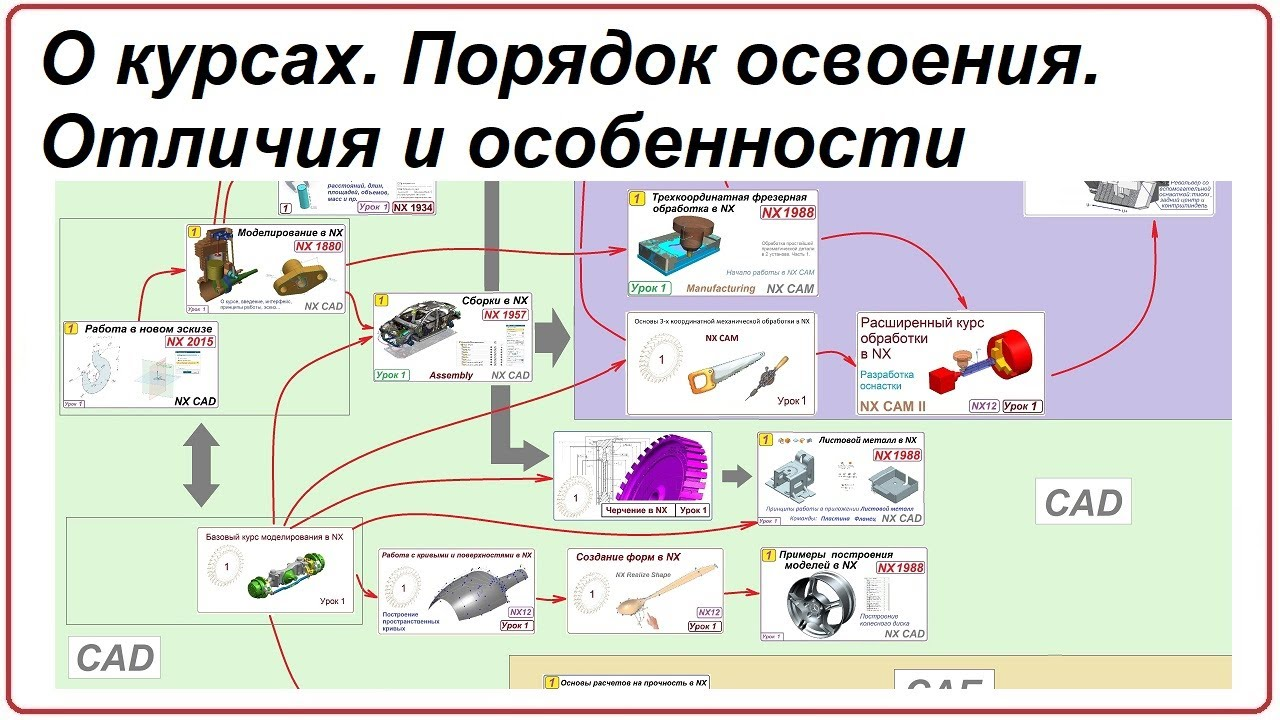
\includegraphics[height=6cm,width=1\textwidth,keepaspectratio]{guidline_preview.jpg}}
        % \caption{Click on a picture for a video}
        \label{fig:guidline_preview.jpg}
    \end{figure}
\end{frame}

\begin{frame}[t]{Assembly Load Options}
    \framesubtitle{Video}
    \vspace{-0.6cm}
    \begin{figure}[H]
        \href{https://disk.yandex.ru/i/k4MD1IFF9-Z1lQ}{
            \centering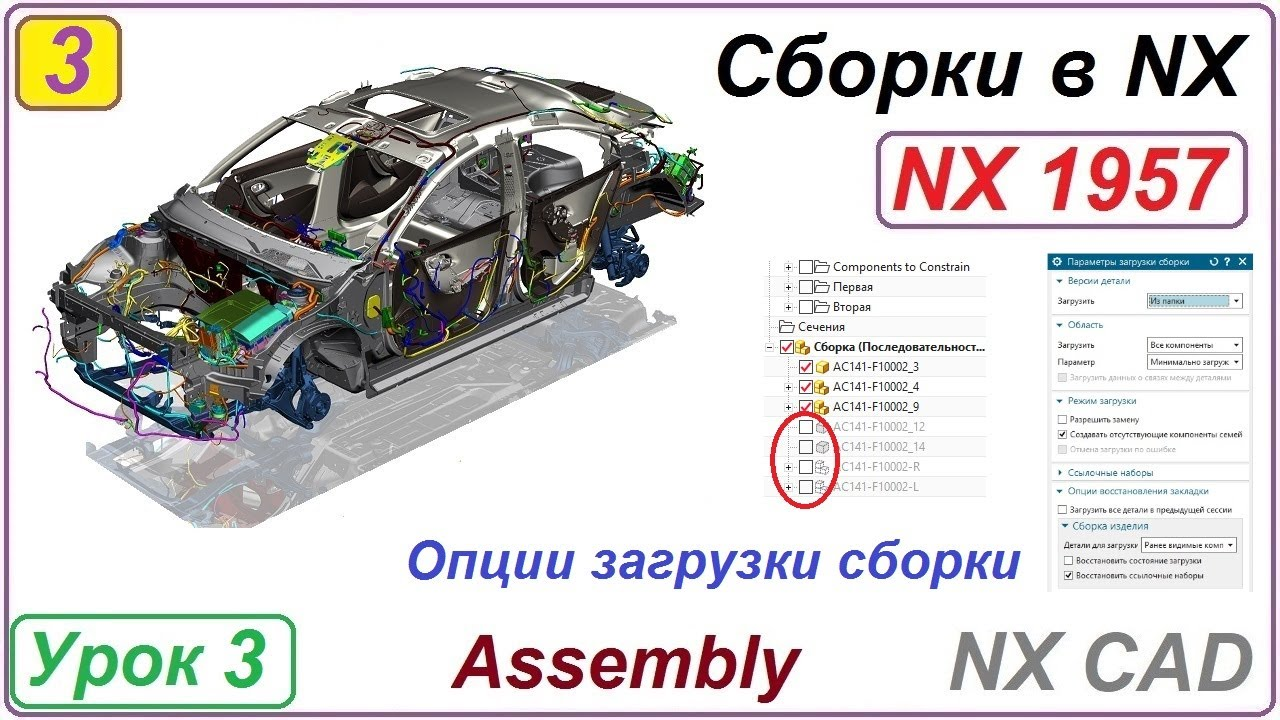
\includegraphics[height=6cm,width=1\textwidth,keepaspectratio]{assembly_load_options_preview.jpg}}
        % \caption{Click on a picture for a video}
        \label{fig:assembly_load_options_preview.jpg}
    \end{figure}
\end{frame}

\begin{frame}[t]{Top-Down Design approach: WAVE}
    \framesubtitle{Video + labs/CAD\_ASM2/task\_data/wave\_tasks.zip}
    \vspace{-0.6cm}
    \begin{figure}[H]
        \href{https://disk.yandex.ru/i/dAw7x_cJdu5VrA}{
            \centering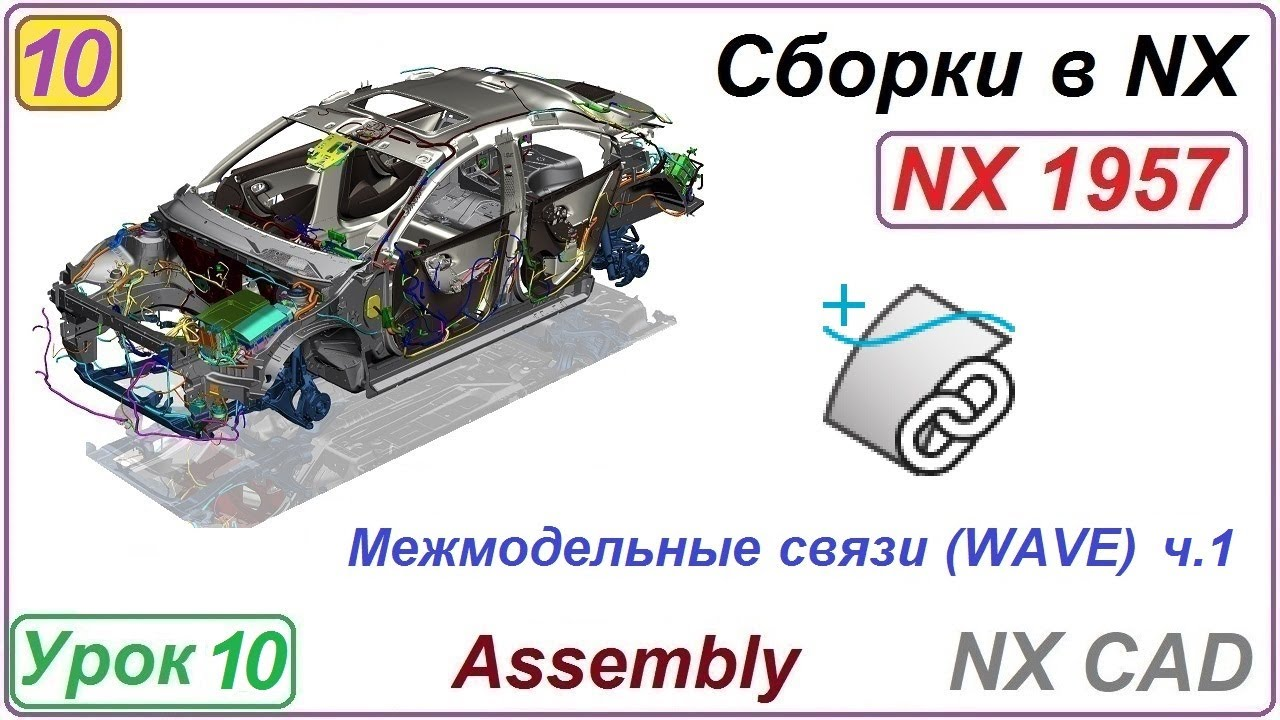
\includegraphics[height=6cm,width=1\textwidth,keepaspectratio]{wave1_preview.jpg}}
        % \caption{Click on a picture for a video}
        \label{fig:wave1_preview.jpg}
    \end{figure}
\end{frame}

\begin{frame}[t]{Practical Task 1}
    \framesubtitle{Make 2 details and assemble them, using WAVE}
    \vspace{-0.6cm}
    \begin{figure}[H]
        \centering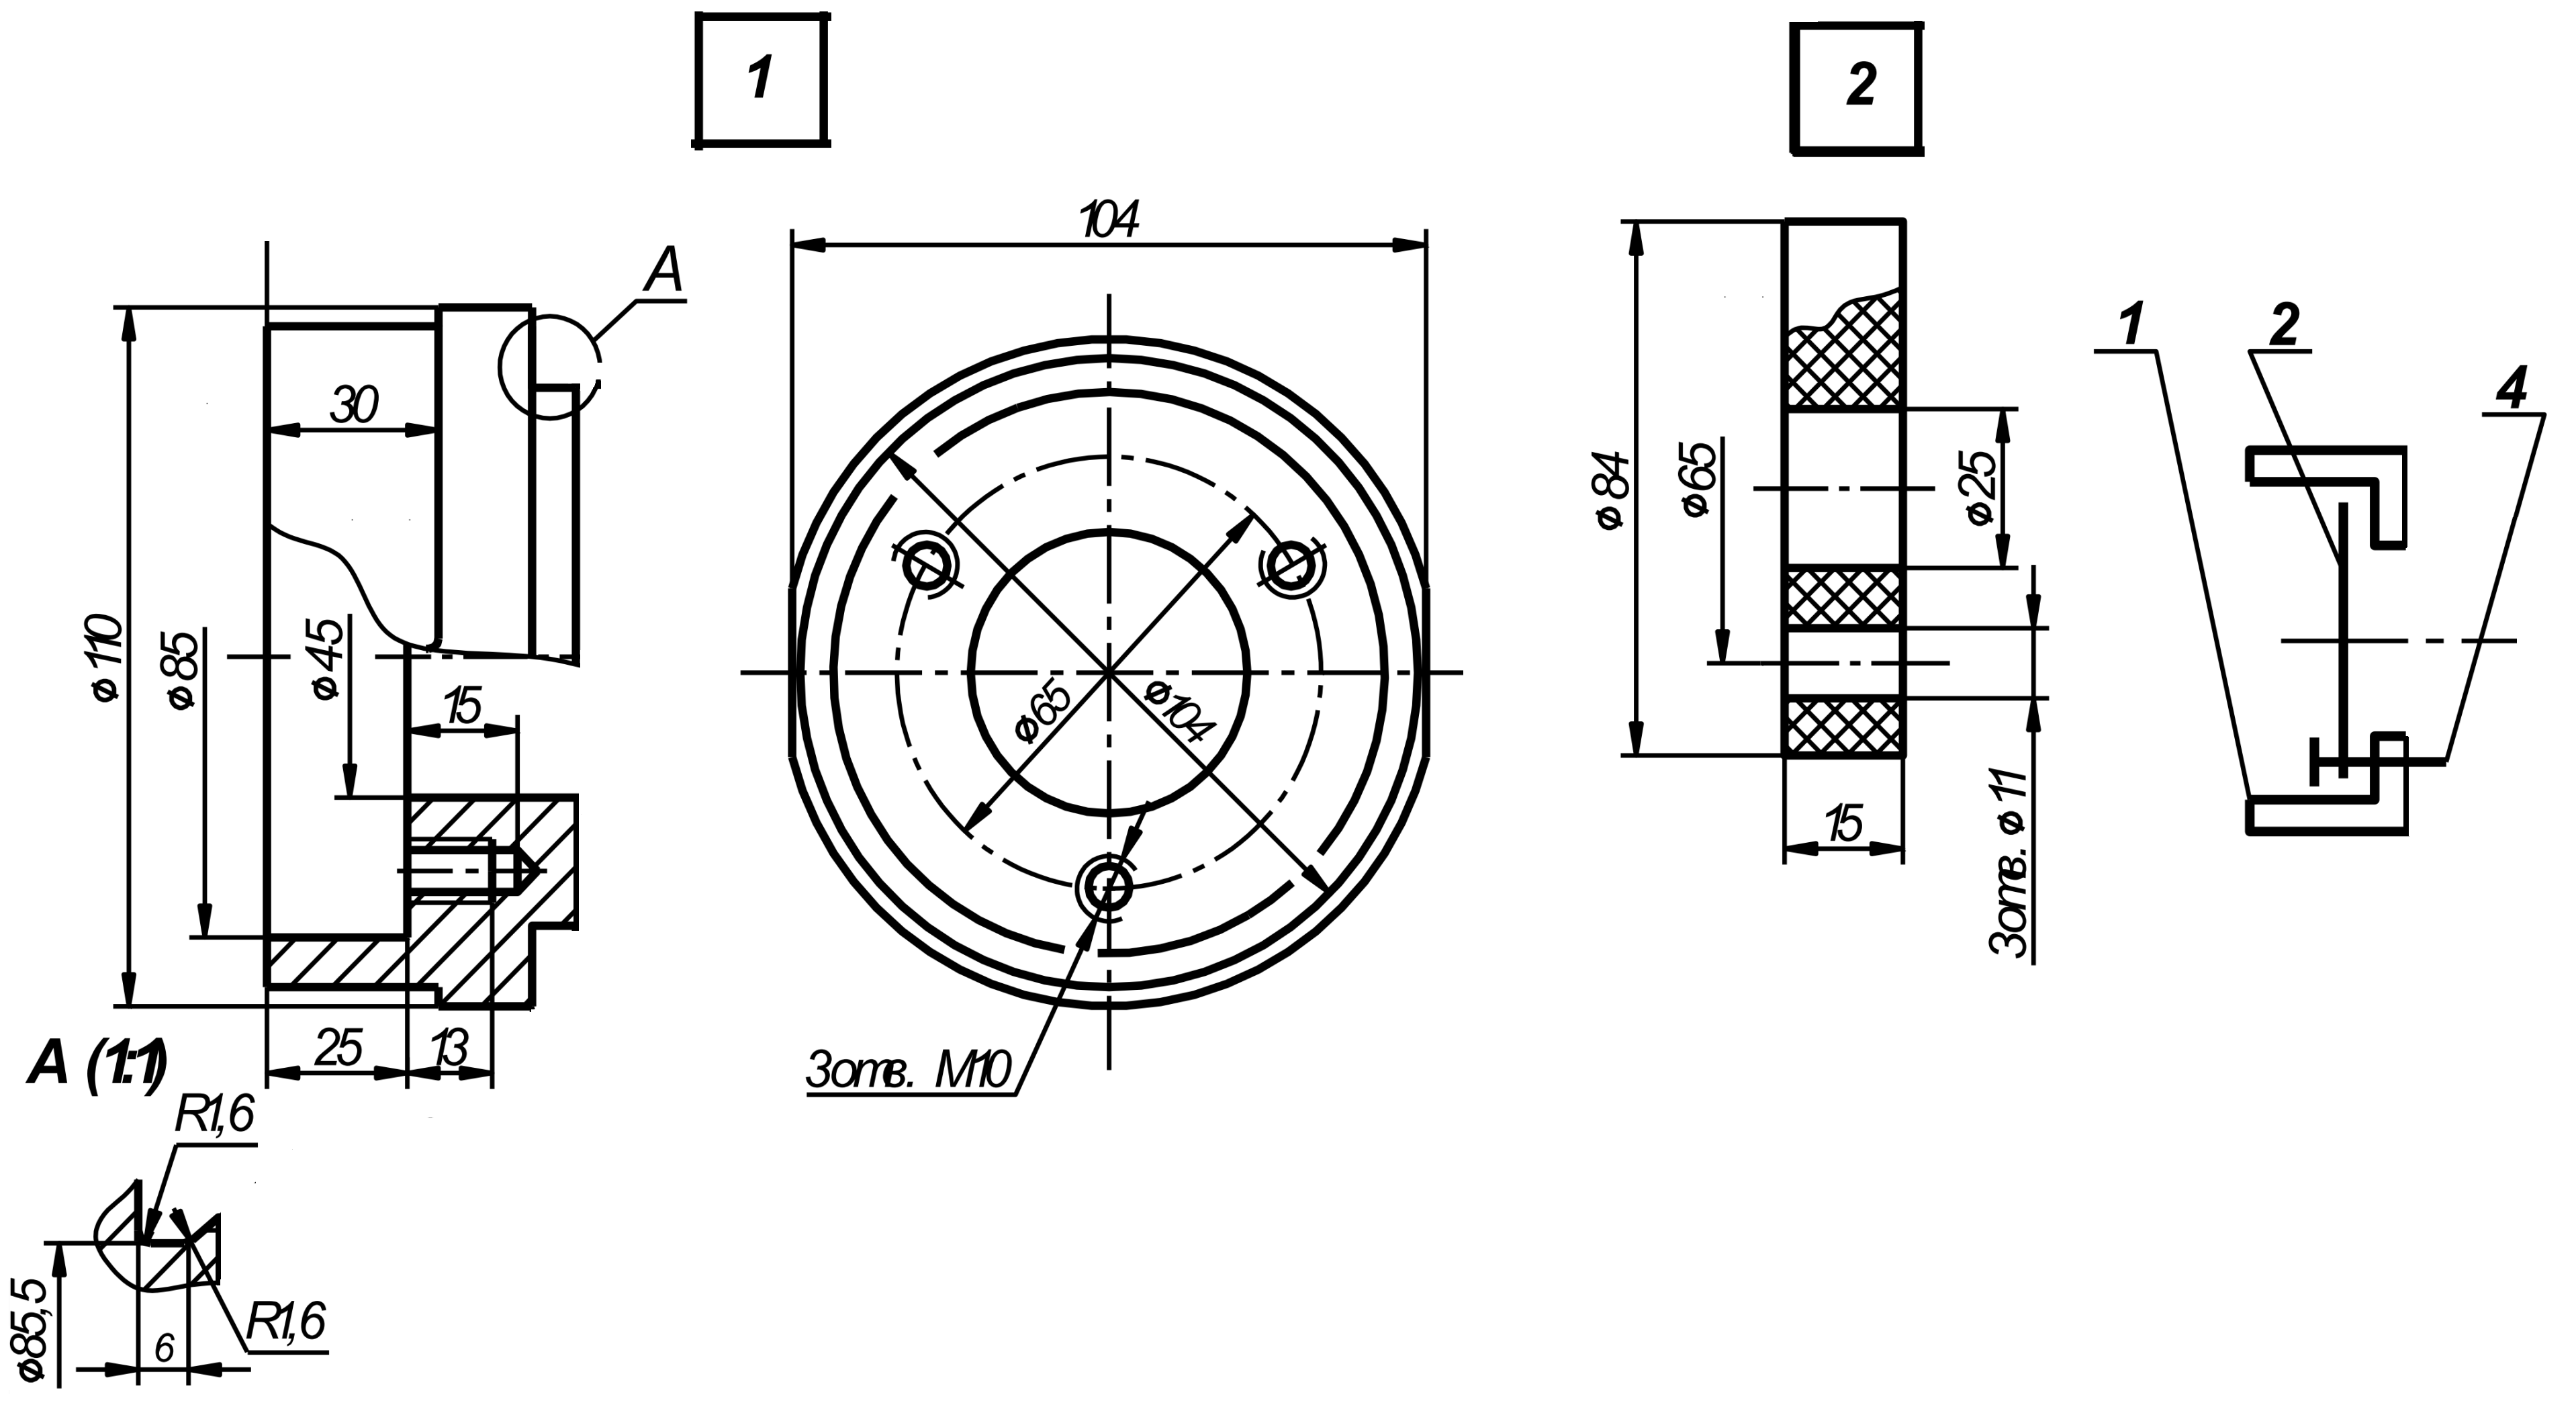
\includegraphics[height=6cm,width=1\textwidth,keepaspectratio]{practical_1.png}
        % \caption{caption_name}
        \label{fig:practical_1.png}
    \end{figure}
\end{frame}

\begin{frame}[t]{Naming conventions}
    \framesubtitle{}
    \vspace{-0.6cm}
    \begin{columns}[T,onlytextwidth]
        \begin{column}{0.55\textwidth}
            The root folder <<<Name>(Part Number)>>.

            \textbf{Subfolders}:
            \begin{itemize}
                \item Information - specifications, descriptions, calculations of inertia, etc.
                \item Pictures - pictures from the project
                \item Components - purchased parts
                \item Simulation - assemblies for which simulation analysis is conducted. The common practice is to make a separate empty assembly, where the necessary part is inserted. This is necessary to reduce the time of loading the part (applicable to Inventor and SolidWorks).
            \end{itemize}

        \end{column}
        \begin{column}{0.44\textwidth}
            \vspace{-1cm}
            \begin{figure}[H]
                \centering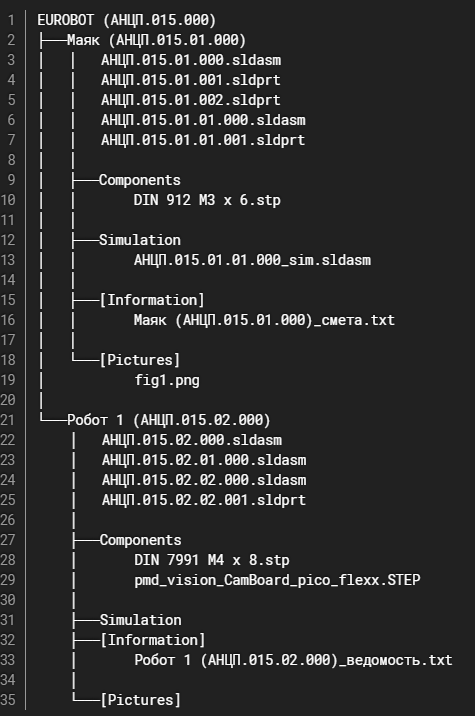
\includegraphics[height=7.2cm,width=1\textwidth,keepaspectratio]{name_1.png}
                % \caption{caption_name}
                \label{fig:name_1.png}
            \end{figure}
        \end{column}
    \end{columns}
\end{frame}

\begin{frame}[t]{Part Number (Обозначение)}
    \framesubtitle{}


    \begin{columns}[T,onlytextwidth]
        \begin{column}{0.49\textwidth}
            It's taken from \href{http://www.robot.bmstu.ru/files/GOST/gost_2.201-80.pdf}{GOST 2.201-80}

            \textbf{Basic rules:}
            \begin{enumerate}
                \item The assembly has 3 zeros at the end of the designation xxxx.xx.000
                \item Part has a number other than zero at the end of the designation e.g. 001, 002
                \item The number of dots indicates the nesting of the assembly or part
            \end{enumerate}
        \end{column}
        \begin{column}{0.49\textwidth}
            \begin{figure}[H]
                \centering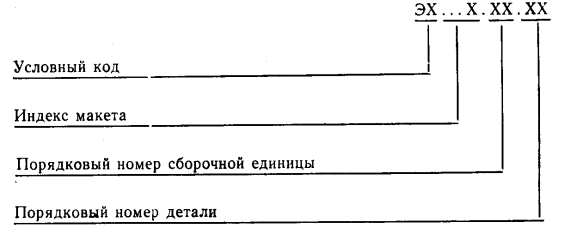
\includegraphics[height=6cm,width=1\textwidth,keepaspectratio]{name_2.png}
                % \caption{caption_name}
                \label{fig:name_2.png}
            \end{figure}
        \end{column}
    \end{columns}
\end{frame}

\begin{frame}[t]{Code Style Guide == GOST naming convention}
    \framesubtitle{}
    \vspace{-0.4cm}
    \begin{enumerate}
        \item Conforming to a style guide removes unneeded guesswork and ambiguities. For example, the full version helps to understand how to manufacture a detail just looked at the name.
        \item It also allows for a more streamlined creation of code and its maintenance, because you \textit{won't have to think about the style or how you should name a variable} --- you simply follow instructions.
        \item If you come to a \textbf{new team}, you \textbf{should follow their style guide --- no questions asked}. You can suggest changes, of course, if you really feel it will be for the better, but otherwise --- just work with their style guide
    \end{enumerate}

    \begin{center}
        Code Style Guide --- team or company level, GOST naming convention --- country level!! \\
        You are \textit{living} in Russia and \textit{have to follow GOST}
    \end{center}
\end{frame}

\begin{frame}[t]{Practical aspects of using namings}
    \framesubtitle{}
    \begin{figure}[H]
        \begin{subfigure}[c]{0.49\textwidth}
            \centering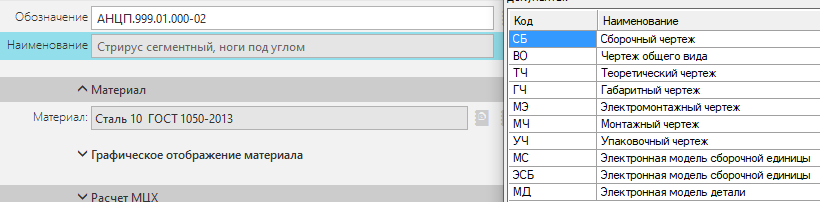
\includegraphics[height=6cm,width=1\textwidth,keepaspectratio]{name_3.png}
            \caption*{KOMPAS 3D}
            \label{fig:name_3.png}
        \end{subfigure}
        \begin{subfigure}[c]{0.49\textwidth}
            \centering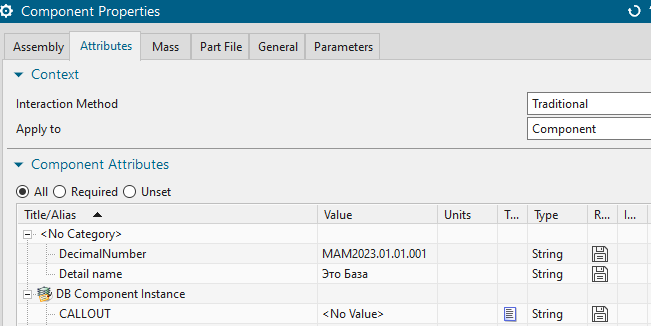
\includegraphics[height=6cm,width=1\textwidth,keepaspectratio]{name_4.png}
            \caption*{Siemens NX}
            \label{fig:name_4.png}
        \end{subfigure}
    \end{figure}
\end{frame}

\begin{frame}[t]{Common Parts Library (Reuse Library)}
    \framesubtitle{}
    \vspace{-0.3cm}

    It's a set of commonly used components (screws, T-slots, etc) for designing and manufacturing device products.

    % \vspace{-0.5cm}
    \begin{figure}[H]
        \begin{subfigure}{0.49\textwidth}
            \centering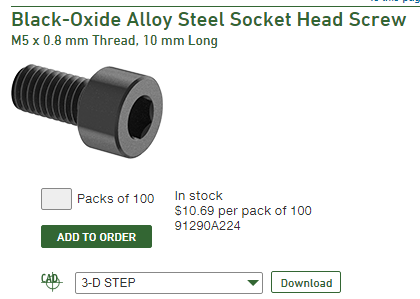
\includegraphics[height=4.5cm,width=1\textwidth,keepaspectratio]{cpl_1.png}
            \caption*{\href{https://www.mcmaster.com/}{McMaster-CARR (from Fusion 360)}}
            \label{fig:cpl_1.png}
        \end{subfigure}
        \begin{subfigure}{0.49\textwidth}
            \centering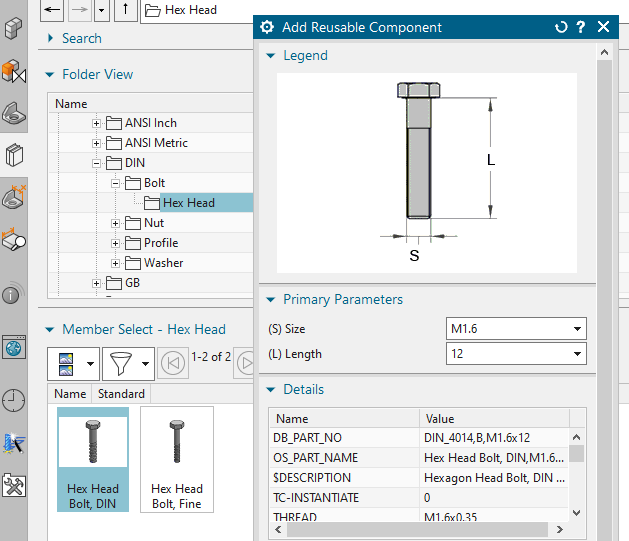
\includegraphics[height=4.5cm,width=1\textwidth,keepaspectratio]{cpl_2.png}
            \caption*{NX Reuse Library}
            \label{fig:cpl_2.png}
        \end{subfigure}
    \end{figure}
\end{frame}

\begin{frame}[t]{Bill of Materials (BOM) (Спецификация) (спека)}
    \framesubtitle{}
    \vspace{-0.5cm}
    \begin{columns}[T,onlytextwidth]
        \begin{column}{0.37\textwidth}
            It is a list of the raw materials, sub-assemblies, intermediate assemblies, sub-components, parts, and the quantities of each needed to manufacture an end product.
            It helps you to:
            \begin{itemize}
                \item Not to forget what do you need to buy and their quantity
                \item To estimate the a manufacturing time
            \end{itemize}
        \end{column}
        \begin{column}{0.61\textwidth}
            \begin{figure}[H]
                \begin{subfigure}[c]{0.49\textwidth}
                    \centering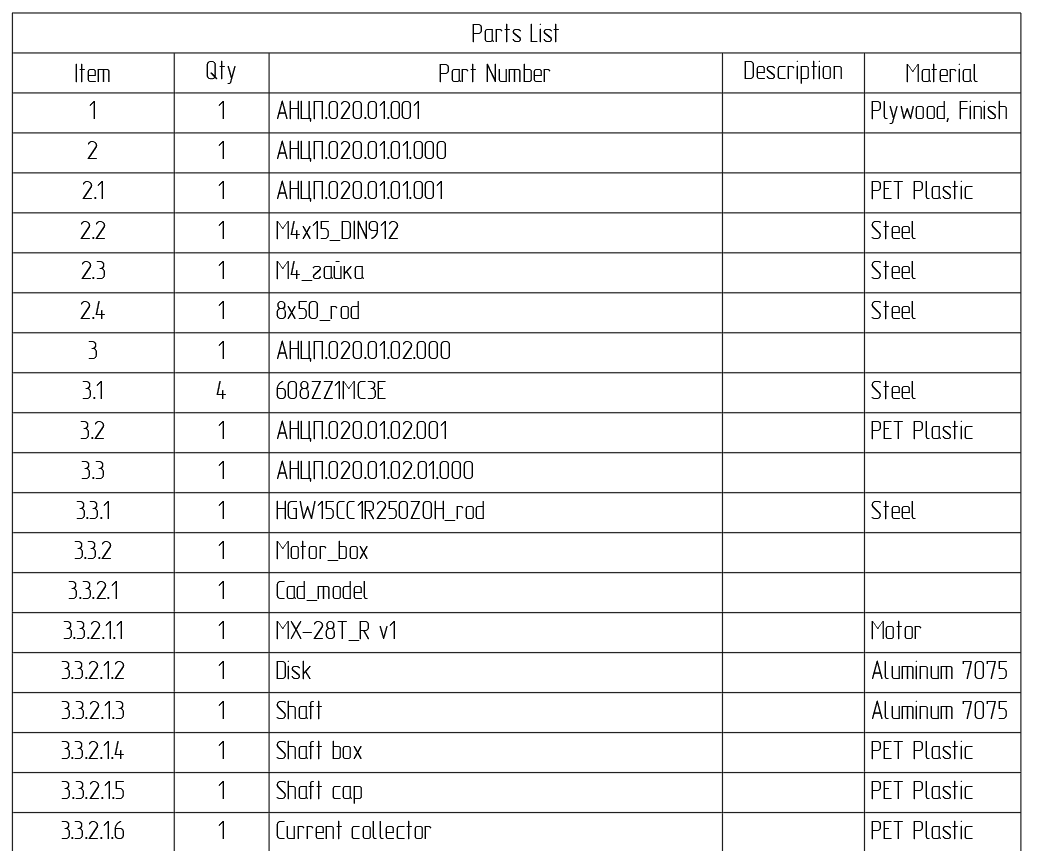
\includegraphics[height=6cm,width=1\textwidth,keepaspectratio]{bom_2.png}
                    \label{fig:bom_2.png}
                \end{subfigure}
                \begin{subfigure}[c]{0.49\textwidth}
                    \centering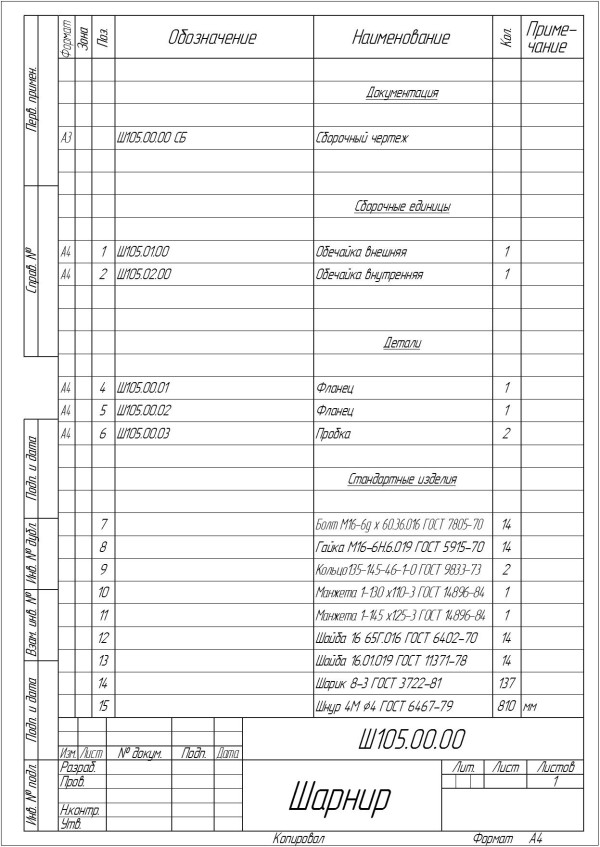
\includegraphics[height=6cm,width=1\textwidth,keepaspectratio]{bom_1.png}
                    \label{fig:bom_1.png}
                \end{subfigure}
            \end{figure}
        \end{column}
    \end{columns}
\end{frame}

\begin{frame}[t]{Bill of Materials in NX}
    \framesubtitle{Video}
    \vspace{-0.6cm}
    \begin{figure}[H]
        \href{https://disk.yandex.ru/i/xTmHh9jwxI5GPw}{
            \centering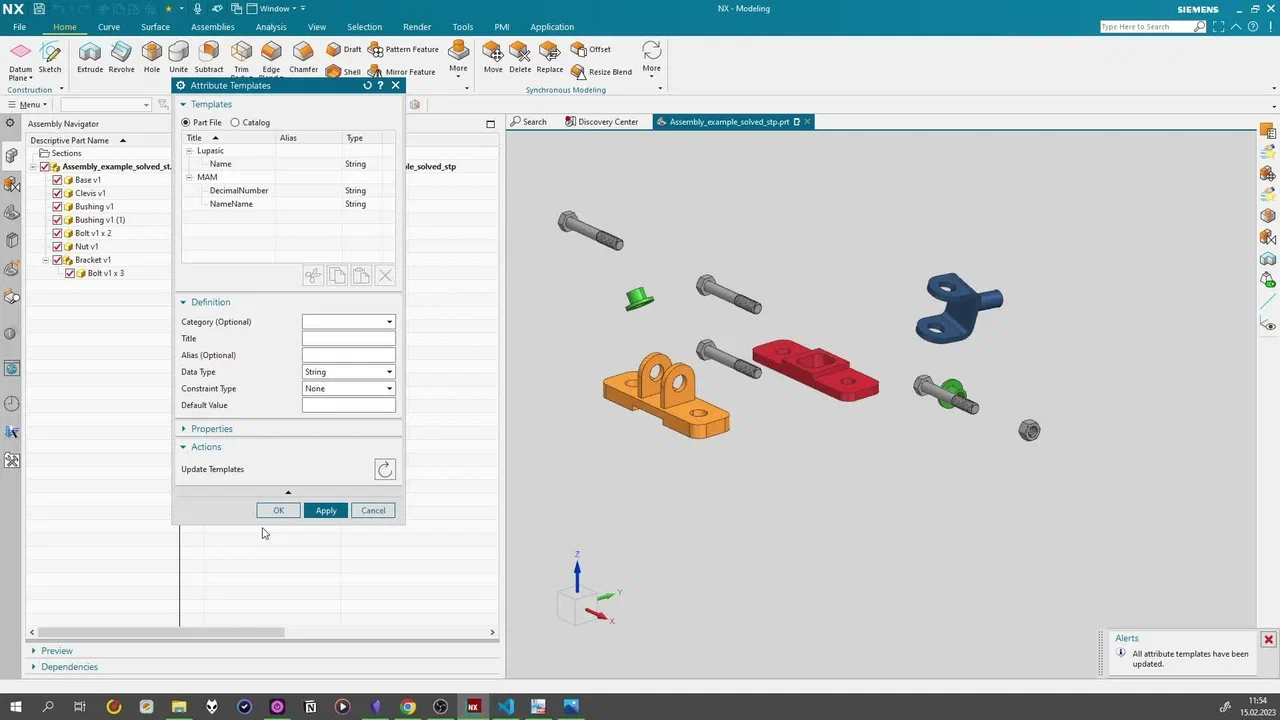
\includegraphics[height=6cm,width=1\textwidth,keepaspectratio]{bom_preview.png}}
        % \caption{Click on a picture for a video}
        \label{fig:bom_preview.png}
    \end{figure}
\end{frame}

\begin{frame}[t]{Sequence (<dis>assembling animation)}
    \framesubtitle{Video + labs/CAD\_ASM2/task\_data/sequence\_task.zip}
    \vspace{-0.6cm}
    \begin{figure}[H]
        \href{https://disk.yandex.ru/i/fDUp5zSG3iDofA}{
            \centering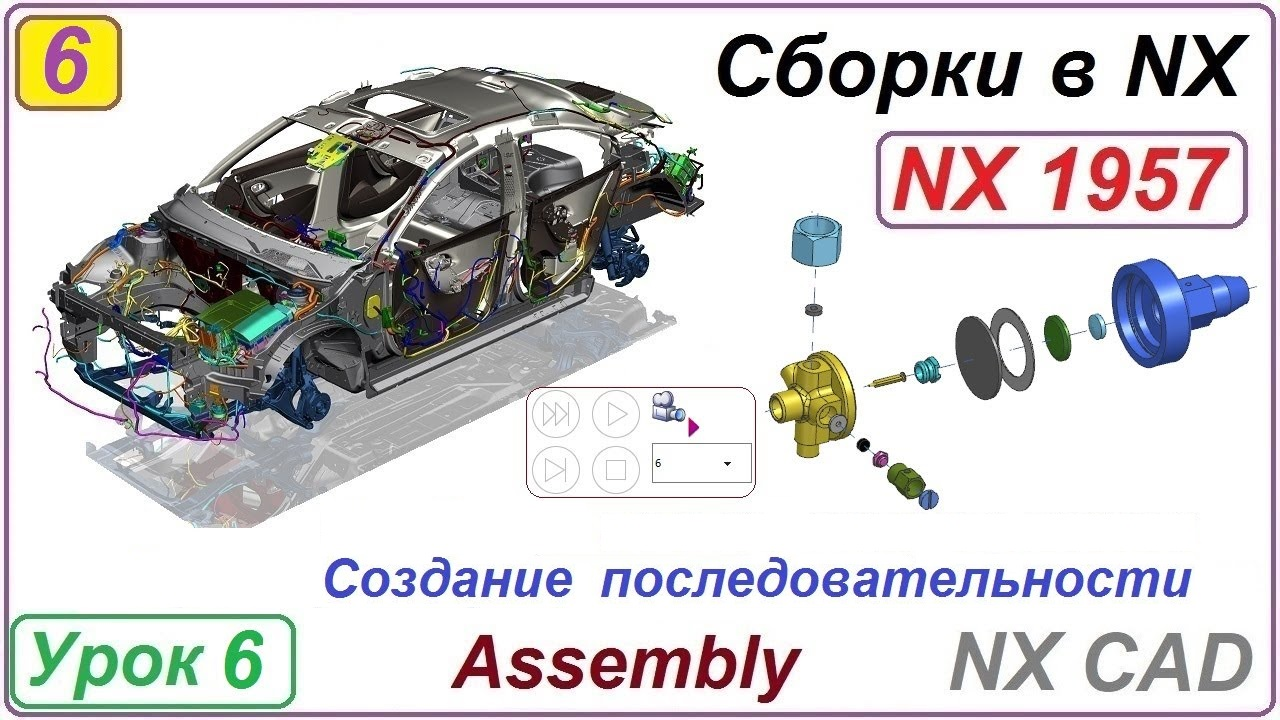
\includegraphics[height=6cm,width=1\textwidth,keepaspectratio]{sequence_preview.jpg}}
        % \caption{Click on a picture for a video}
        \label{fig:sequence_preview.jpg}
    \end{figure}
\end{frame}

\fbckg{fibeamer/figs/last_page.png}
\frame[plain]{}

\end{document}